%*****************************************************************************************
\chapter{Analysis of Current System}
\ifpdf
    \graphicspath{{Chapter2/Figs/Raster/}{Chapter2/Figs/PDF/}{Chapter2/Figs/}}
\else
    \graphicspath{{Chapter2/Figs/Vector/}{Chapter2/Figs/}}
\fi

%%%%%%%%%%%%%%%%%%%%%%%%%%%%%%%%%%%%%%%%%%%%%%%%%%%%%%%%%%%%%%%%%%%%%%%%%%%%%%%
\section{Introduction}

This part of the project can be outlined as follows:

\begin{itemize}
    \item Collect data sets on which a machine learning classifier is to be trained
    \item Construct a program capable of processing and storing such data sets
        such that required subsets of the data can be quickly and easily
        returned for further analysis
    \item Select a suitable machine learning framework to handle the training
        and validation of a classifier
    \item Ensure a robust validation methodology exists for assuring quality of
        our own results
    \item Set up an environment capable of allowing results from such a
        classifier to be stored and compared
    \item Training a suitable classifier on the collected data sets
    \item Perform experiments by selecting subsets of the variables and
        observations and measure whether classification accuracy is improved
\end{itemize}

%%%%%%%%%%%%%%%%%%%%%%%%%%%%%%%%%%%%%%%%%%%%%%%%%%%%%%%%%%%%%%%%%%%%%%%%%%%%%%%
\section{Materials and Methods}
\subsection{Input Data and Format}

%NOTE Assuming lanelets have been described by this point...
%TODO samtools stats actually generates this data rather than "the seq process"
As part of the project I've been granted access to significant data sets at the
Sanger Institute, unlocking quality control data for two of the largest studies
currently undergoing analysis. A wide array of quality metrics are available for
each and every lanelet that forms part of either of the two studies; totalling
13,455 files.

%9154 (68\%), 1542 (11\%), 2759 (21\%)...

%TODO Citation for samtools?
%TODO Explain a BAM file
The files are created by \textbf{samtools stats} --- part of a collection of
widely used open-source utilities for post processing and manipulation of large
alignments such as those produced by next-generation sequencers that are
released under the umbrella name of "SAMtools" (Sequence Alignment and Map
Tools). \textbf{samtools stats} collects statistics from sequence data files %BAM
and produces key-value summary numbers as well as more complex tab delimited
dataframes tabulating several metrics over time.

%TODO Was samtools stats known as bamcheck, or did it replace it?
The output of \textbf{samtools stats} is then parsed by an in-house tool called
\textbf{bamcheckr}, named so as \textbf{samtools stats} was once known as
\textbf{bamcheck} and the tool is written in R. \textbf{bamcheckr} supplements
the summary numbers section of the \textbf{samtools stats} output with
additional metrics that are later used by \textbf{auto\_qc} for classification.
This process does not change the file other than adding a few additional
key-value pairs in the summary numbers section. A truncated example of a
"bamcheckr'd" file can be found in Appendix~\ref{AppendixA}.


%%%%%%%%%%%%%%%%%%%%%%%%%%%%%%%%%%%%%%%%%%%%%%%%%%%%%%%%%%%%%%%%%%%%%%%%%%%%%%%
\subsection{Development Environment}
\subsubsection{Language}
%TODO Better opening
%TODO Do I need to ramble about why vim is great and so on?
For the language of the program designed to handle this vast array of input
data, Python was selected, more out of personal taste rather than a
detailed analysis of required performance and features. From previous experience
I was happy with the performance of Python when processing large datasets in
terms of both I/O file handling operations and storing the data in memory for
later use. Python's generous choice of both built-in and third-party libraries
have proven useful on many occasions. Due to its concise and flexible nature it
is possible to rapidly develop applications and its readability eases ongoing
maintenance; useful given the short time-span allocated for this project and the
possibility of others wishing to contribute to the project codebase after
completion.

%TODO Pushing WEKA too much with "certainly"?
Whilst the choice was made primarily on preference, this is not to say other
options were not considered: a highly popular Java-based collection of data
mining tools, \textbf{WEKA} would certainly have provided a framework for
building decision tree classifiers but at the same time did not appear to offer
any significant features that were unavailable elsewhere, whilst Java itself has
the added constraint of requiring a virtual machine to be installed which could
be undesirable from a performance or even security standpoint when the
application is deployed to servers at the Sanger Institute.

%...although performance has improved considerably from previous Java versions\citep{Bouckaert}

Difficulty was also encountered finding example implementations for \textbf{WEKA}
with most documentation and tutorials providing information for performing
analysis via the graphical "Explorer" interface instead, which would not be
appropriate for quickly setting up and repeating experiments automatically.

%TODO Link to http://cran.r-project.org/web/packages/tree/tree.pdf
Given the quality data we'll be using to train a machine learning classifier is
output from the previously mentioned R script; \textbf{bamcheckr}, it was worth
briefly investigating the options available for R itself as the potential of
integrating the learning and predicting functions right in to the same process
that outputs the data seemed convenient.

...Whilst the \textbf{tree} and \textbf{rpart} packages are available for
constructing decision trees in R but (and actually \textbf{RWeka} provides an R
interface to \textbf{WEKA})...they did not appear to be as robust as
other more well-known frameworks. Putting it politely, the programming paradigm
of R is rather different to other languages and can significantly increase
development time if one is not very well versed in the patterns and grammar of
the language and it seemed best to stick to one's comfort zone.

...C and C++ also a possibility, however \textbf{dlib} didn't support tree-based
classifiers although \textbf{Shark} did, Python chosen in the end for ease of
use...


\subsubsection{Framework}
...Having studied the Machine Learning module in final year the prospect of
getting stuck in to the deep of a machine learning algorithm was exciting,
however the reality is a lot of time and effort has gone in to proper
optimisation of a framework which is unlikely to be surpassed successfully by a
short-term one-person project. It is therefore only natural that a library seems
a wise investment for the codebase...

...There are numerous machine learning frameworks available in many languages,
some described above... however it seemed counter-intuitive to select a
framework in another language for the introduction of an additional arbitrary
output and input steps to switch between the two environments.

...A mixed bag of such frameworks exist in Python, two in particular
\textbf{scikit-learn} and \textbf{Orange} were main contenders, partly on their
recommendation from the project supervisor...

...scikit integrates the "big names" in Python: numpy, scipy and matplotlib
...put off from Orange due to difficulties in reading in data ...it did however
later appear to ship with features that were not in scikit (pruning and
printing) ...with more time I'd certainly like to investigate using other
libraries such as \textbf{Orange} or even outside Python and take at look at WEKA
or Shark...

\subsubsection{Libraries}
numpy, scipy... Fast and reliable implementations of
mathematical functions...  ggplot2 for beautiful graphing...

\subsubsection{Testing}
Investigated the possibility of using \textbf{Jenkins}
but just didn't have the time to set up and tweak all the plugins and options of
the platform to do what I wanted... Would still have been poor in terms of
searching through logs to track what parameters led to improvements in cross
validation... ...Quite likely I'd have needed to author a Java or Groovy plugin
to keep good track of cross-validation...

Briefly considered online solutions such as \textbf{Travis} and \textbf{Wercker}
which I use for some personal projects, whilst quicker to set up would probably
have not been able to handle artifacts such as dot files without some convoluted
solution of uploading them to dropbox or adding them to a private git repository
from the build node...  ...also would have needed to upload a very large
quantity of training data repeatedly which would be inefficient (and more than
likely against reasonable use of the platform)

Really wanted to write my own solution for this but had to settle for well
formatted log files that could be searched and processed with some command line
fu...

\subsubsection{Additional Tools}
Version control is critical, \textbf{git}!


%%%%%%%%%%%%%%%%%%%%%%%%%%%%%%%%%%%%%%%%%%%%%%%%%%%%%%%%%%%%%%%%%%%%%%%%%%%%%%%
%TODO Rubbish section title
\section{Pre-Implementation}
\subsection{Classification Correlation}
...An important consideration for statistical analysis is the relation between the
observations. The quality data files we have are per lanelet, however a lane can
house more than one lanelet...  and so herein lies the trouble, if during a run,
the flow cell is somehow subjected to abnormal temperatures (air conditioning
failure) or the sequencing device is depleted of reagents, every lane (and thus
lanelet within) will be of very poor quality. Thus there would appear to exist a
relationship between the respective qualities of each lanelet in a lane as well
as each lane in a sequencing run!

%TODO Probably mention in the text this is a very dense heatmap...
\begin{figure}[htbp!]
    \centering
    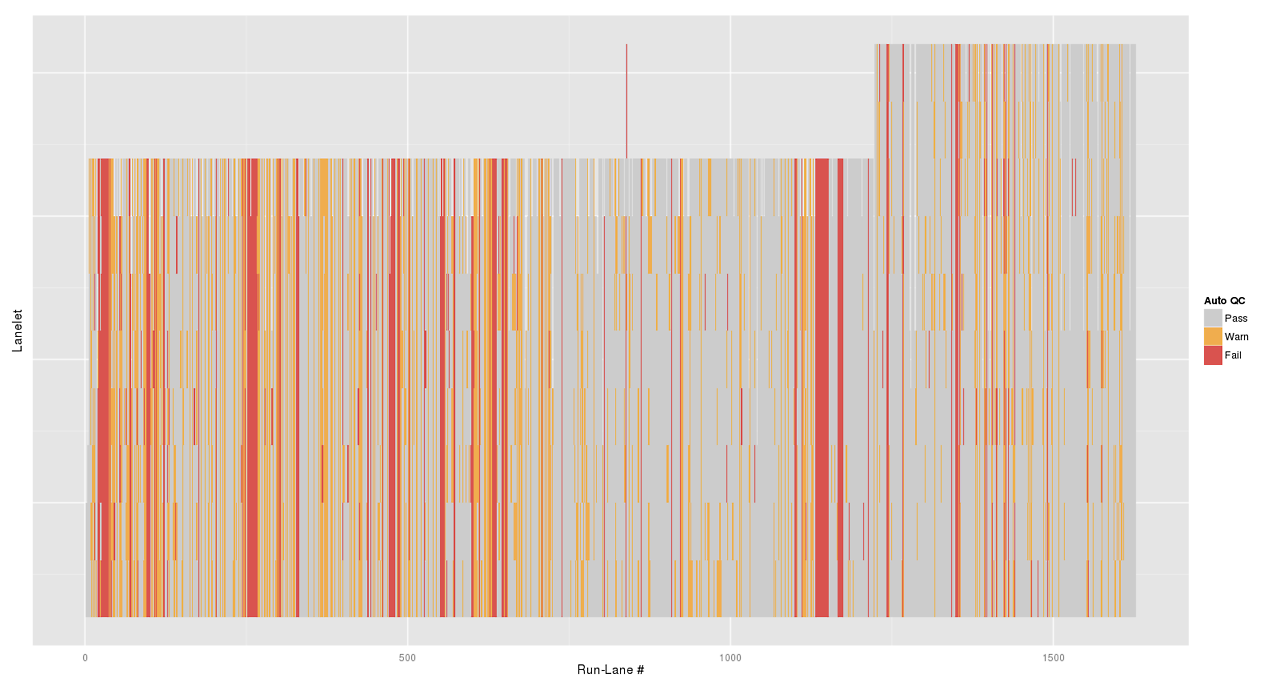
\includegraphics[width=1.0\textwidth]{classcorr}
    \caption[ClassCorr]{Heatmap of Lanelet QC Status by Lane}
    \label{fig:classcorr}
\end{figure}

%TODO Throwing in the word library
...Figure~\ref{fig:classcorr} displays a plot of auto\_qc classification for
each lanelet (y) versus lane (x). ...The plot was designed to be a diagnostic
test to see whether this was the case. I should mention that it seems there are
few conditions under which a lanelet would fail irrespective of the auto\_qc
status of the rest of the lanelets in the lane; which mostly involve the
preparation of the sample (which is easy to spot given it will cause poor
quality across all lanelets using that library sample).

...an unbroken vertical red bar indicates that all the lanelets inside a
particular lane failed. Likewise yellow represents a warning. Grey areas are
passes and were desaturated to make the other outcomes immediately obvious. It
is clear that there are patches where lanelets have failed where entire lanes
have not, but there does appear to be some correlation.

%TODO
Having discussed this with the supervisor and contacts at the Sanger Institute
we decided to continue...

Note the plot does not make a particular distinction between lanes in the same
flow cell but they are sequentially identified so the red bars of thicker-width
arguably display some failures across entire flow cells.

%%%%%%%%%%%%%%%%%%%%%%%%%%%%%%%%%%%%%%%%%%%%%%%%%%%%%%%%%%%%%%%%%%%%%%%%%%%%%%%
\section{Implementation}
\subsection{Frontier}
\textbf{Frontier} is the programmatic output for this part of the project...
providing an API-like interface to the data itself... ...allowing simple
commands to pull the data out from memory in to formats aceptable by the machine
learning framework...

...provides a class to read from the "bamcheck files" as seen in
Appendix~\ref{AppendixA}...

...a major refactoring to remove hard-coded classes from \textbf{Frontier} which
enable it to be used as a more general purpose tool; if we were to add another
class label, the definition would merely need to be included to the CLASSES
(Fig~\ref{fig:FrontierClasses}) variable passed when the Statplexer is
constructed. But use is therefore not merely limited to our problem but rather
any machine learning problem where you'd like to simplify your interactions
which a very large dataset.

\begin{minted}[mathescape,
               %linenos,
               numbersep=5pt,
               gobble=2,
               frame=lines,
               framesep=2mm]{python}
    CLASSES = {
            "pass": {
                "class": ["pass"],
                "names": ["pass", "passed"],
                "code": 1,
            },
            "fail": {
                "class": ["fail"],
                "names": ["fail", "failed"],
                "code": -1,
            },
            "warn": {
                "class": ["warn"],
                "names": ["warn", "warning"],
                "code": 0,
            },
    }
\end{minted}

\subsubsection{Cross Validation}
...K fold cross validation
...stratified cross validation...

\subsubsection{Confusion Matrices}

\subsection{Contributions to bamcheckr}
\begin{minted}[mathescape,
               %linenos,
               numbersep=5pt,
               gobble=2,
               frame=lines,
               framesep=2mm]{r}
    install.packages("devtools")
    library(devtools)
    install_github("samstudio8/seq_autoqc", subdir="bamcheckr")
\end{minted}

...R CMD BATCH issue

...Fixed a graph plotting failure.
...Writing additional routines...

%%%%%%%%%%%%%%%%%%%%%%%%%%%%%%%%%%%%%%%%%%%%%%%%%%%%%%%%%%%%%%%%%%%%%%%%%%%%%%%
\section{Results}
\subsection{Initial Trees}
\subsection{Parameter Sets}
